

\begin{frame}
\frametitle{Fault modelling and safety design patterns}
\begin{itemize}
  \item Faults injection to find failures---it's an important approach to discover hidden faults combination;
  \item Fault modelling is a more detailed approach, to let a designer model nominal behaviour and erroneous behaviour at the same time.
  \item Two approaches analyse system safety: fault injection and fault modelling 
\end{itemize}
\end{frame}

\begin{frame}[fragile]
\frametitle{Analyse system safety with fault injection}

\begin{itemize}
  \item From traces
\begin{snippetcspm}[0]
TRACE 1:
failure.Hardware.N04_MonIn2.1.EXP.I.5
failure.Hardware.N04_MonIn2.1.ACT.OMISSION
failure.Hardware.N04_RelationalOperator.1.EXP.B.true
failure.Hardware.N04_RelationalOperator.1.ACT.B.false
out.1.OMISSION

TRACE 2:
failure.Hardware.N04_MonIn1.1.EXP.I.5
failure.Hardware.N04_MonIn1.1.ACT.OMISSION
failure.Hardware.N04_MonIn2.1.EXP.I.5
failure.Hardware.N04_MonIn2.1.ACT.OMISSION
out.1.OMISSION
\end{snippetcspm}
  \item We obtain \emph{lists} $[B,S]$, $[A,B]$---a finite set of lists
  \item We need an algebra to reduce the set of lists 
\end{itemize}
\end{frame}

\begin{frame}
\frametitle{Inspiration: Free Boolean Algebra}
\begin{itemize}
  \item Free variables: A, B, C, \ldots
  \item Any Boolean formula in Free Boolean Algebra (FBA) is written as a set of sets
    \begin{itemize}
      \item For an algebra with three variables $\{A,B,C\}$
      \item $A \lor B =_{\fba} \{ \{A\}, \{B\}, \{A,B\}  \}$
      \item $\lnot A =_{\fba} \{ \{\,\}, \{B\},\{C\},\{B,C\}  \} $
    \end{itemize}  
  \item In Isabelle/HOL, the AFP has a theory to formalize FBAs
  \item An inductive set ($\fba$) defines a set of all possible formulas

\end{itemize}
\end{frame}

\begin{frame}
\frametitle{Free Boolean Algebra}
Given the inductive set $\fba$
\begin{subequations}
\begin{align}
\{F | i \in F \} & \in \fba & \text{(Variable)}\\
S \in \fba \implies -S & \in \fba & \text{(Complement)}\\
S \in \fba \land T \in \fba \implies S \inter T & \in \fba & \text{(Intersection)}
\end{align}
\end{subequations}

The Boolean algebra elements ($\top$, $\bot$) and operators ($\lor$, $\land$, $\lnot$) are defined:
\begin{itemize}
  \item $\top =_{\fba} UNIV$ (all sets of free variables combinations)
  \item $\bot =_{\fba} \{\}$
  \item $A =_{\fba} \{F | A \in F\} $
  \item $A \land B =_{\fba} \{F | A \in F \} \inter \{F | B \in F\}$ 
  \item $A \lor B =_{\fba} \{F | A \in F \} \union \{F | B \in F\}$
  \item $\lnot A =_{\fba} - \{F | A \in F\}$
\end{itemize}
\end{frame}

\begin{frame}
\frametitle{Temporal Faults Algebra}

\begin{itemize}
  \item Free Variables
  \item Any formula is written as a set of lists
    \begin{itemize}
      \item For an algebra with three variables $\{A,B,C\}$
      \item $A \lor B =_{\tfa} \{ [A], [B], [A,B], [B,A], [A,B,C], [A,C,B], \ldots, [C,B,A]  \}$
      \item $\lnot A =_{\tfa} \{ [\,], [B], [C], [B,C], [C,B] \} $
      \item $A \xbefore B =_{\tfa} \{ [A,B] \}$
    \end{itemize}  
  \item An inductive set ($\tfa$) defines a set of all possible formulas
\end{itemize}
\end{frame}

\begin{frame}
\frametitle{Temporal Faults Algebra}

$\tvar x = \{l | \distinct l \land x \in \set l\}$
%
\begin{subequations}
\begin{align}
%
\tvar x &\in \tfa & \text{Variable}\\
%
S \in \tfa \implies \{ l | l \in -S \land \distinct l\} &\in \tfa & \text{Negation}\\
%
S \in \tfa \land T \in \tfa \implies 
S \inter T &\in \tfa & \text{Intersection} \\
%
S \in \tfa \land T \in \tfa \implies 
S \rightarrow T & \in \tfa & \text{Exclusive before }
%
\end{align} %
%
\end{subequations}%

The Boolean algebra elements ($\top$, $\bot$) and operators ($\lor$, $\land$, $\lnot$) are defined:
\begin{itemize}
  \item $\top =_{\tfa} \{l | \distinct l\}$ (all sets of distinct lists)
  \item $\bot =_{\tfa} \{\}$
  \item $A =_{\tfa} \tvar A $
  \item $A \land B =_{\tfa} \tvar A \inter \tvar B$
  \item $A \lor B =_{\tfa} \tvar A \union \tvar B$
  \item $\lnot A =_{\tfa} \{l | l \in - \tvar A \land \distinct l\}$
\end{itemize}
\end{frame}

\begin{frame}{Exclusive before definition}
\begin{align*}
S \rightarrow T = &\left\{ l \bullet \exists xs, ys | xs \in (S - T) \land ys \in (T - S) \land \right.
%
\\& \left. distinct (xs \concat ys) \land l = xs \concat ys \right\}
\end{align*}

Example:
\begin{align*}
\tvar a =& \left\{[a],[a,b],[b,a],[a,c],[c,a],[a,b,c],\ldots,[c,b,a]\right\} \\
\tvar b =& \left\{[b],[a,b],[b,a],[b,c],[c,b],[a,b,c],\ldots,[c,b,a]\right\} \\
\tvar a \rightarrow \tvar b =& \left\{[a,b],[a,b,c],[a,c,b],[c,a,b]\right\}
\end{align*}

\end{frame}

\begin{frame}
\frametitle{Temporal Faults Algebra -- Isabelle/HOL}
\includeautosizegraphics{tformula-01}

\onslide<2>{%
\tikzoverlay[text width=6.5cm] at (4.5cm,5.5cm) {%
$a \tformulat = tfa :: a \listt \sett \sett $\\
$Abs\_\tformulat :: a \listt \sett \sett \Rightarrow a \tformulat $\\ 
$Rep\_\tformulat :: a \tformulat \Rightarrow a \listt \sett \sett $%
};
}
\end{frame}

\begin{frame}
\frametitle{Temporal Faults Algebra -- Isabelle/HOL}
\includeautosizegraphics{tformula-02}
\end{frame}

\begin{frame}
\frametitle{Safety analysis using structure function}

\begin{itemize}
  \item Qualitative analysis:
    \begin{itemize}
      \item Obtaining minimal cut sets -- sets of events that cause the top fault event \onslide<2->{-- Rule: \alert<2>{$\BasicEventMinLevel$}}
      \item Importance analysis -- cut sets with fewer events are more important
      \item Minimal cut sets susceptible to common cause failures
    \end{itemize}
  \item Quantitative analysis:
    \begin{itemize}
      \item Absolute probability of the top event \onslide<2->{-- Rule: \alert<3>{$\RootProbability$}}
      \item Quantitative component importance -- percentage of time that a system failure is caused by a particular minimal cut set
      \item Effects of changing maintenance and checking time, implementing design modifications or changing component reliabilities
    \end{itemize}
\end{itemize}
\end{frame}

\begin{frame}
\frametitle{Fault Tree Rule evaluation (or acceptance criteria)}


Function $\evaluateRule$ is defined as:
$\evaluateRule :: FaultTree \Rightarrow FaultTreeRule \Rightarrow Probability \Rightarrow bool$
{
\footnotesize 
\begin{subequations}
\begin{align}
\evaluateRule ft \, (\BasicEventMinLevel n) P &= (\minBasicEventLevel ft \ge n)\\
\evaluateRule ft \, (\RootProbability p) P &= (\ftProbability ft \, P) \le p
\end{align}
\end{subequations}
}

Function $\minBasicEventLevel$ is defined as $0$ if the structure expression is a variable or $1$ plus the minimum of $\minBasicEventLevel$ of the subexpressions.
%
Function $\ftProbability$ calculates the probability of an expression, given the probability of basic events (variables). Ex.: $\ftProbability (A \lor B) P = P(A) + P(B) - P(A) \times P(B)$
\end{frame}

\begin{frame}
\frametitle{Fault modelling}

\begin{itemize}
  \item By component. Ex.: if fault $\failurevalue{A}{1}$ occurs in some component $\component{1}$, the output is $\outvalue{U}{1}$, if fault $\failurevalue{B}{1}$ occurs, the output is $\outvalue{V}{1}$, otherwise, the output is nominal.
  \item Interface-focused. Ex.: if component $\component{2}$ is connected in its input port $1$ to component $\component{1}$, then if $\component{2}$ observes some fault $\failurevalue{A}{1}$ in input port $1$ caused by $\component{1}$, then $\component{2}$ output is $\outvalue{U}{2}$, otherwise the output is nominal.
\end{itemize}

\end{frame}

\begin{frame}
\frametitle{Activation Algebra for fault modelling}
\begin{itemize}
  \item Faults are variables in some algebra ($\failurevalue{A}{1} = \failurevalue{\text{Internal failure}}{1}$, $\failurevalue{A}{2}=\failurevalue{\text{Internal failure}}{2}$)
  \item Each operand is a pair: (i) an expression in some algebra (Boolean or Temporal), and (ii) an output value.
  \item Output values are identified by: (i) a failure mode and optionally a numerical value (ex.: $\outvalue{U}{1}$ = Omission), or (ii) $N$ and a numerical value to express a nominal value. 
  \item Ex.: $exp = \aaexp{\alert<2>{\failurevalue{A}{1}}}{\alert<4>{\outvalue{U}{1}}} \alert<2>{\lor} \aaexp{\alert<2>{\lnot \failurevalue{A}{1}}}{\nominalvalue{5}{1}}$
  \item<2-> The expressions of the algebra when combined should give a tautology: $\failurevalue{A}{1} \lor \lnot \failurevalue{A}{1} = \top$
  \item<3-> Predicate:
  $P\left(exp\right) \defs \alert<4>{\outvalueof{exp}=\outvalue{U}{1}} \iff 
  %
  P\left(exp\right) = \failurevalue{A}{1}$
  \item<4-> We then use the predicates in the given algebra to apply Fault Tree Rules
\end{itemize}
\end{frame}

\begin{frame}
\frametitle{Activation Algebra for our example}

\begin{itemize}
  \item $\failurevalue{S}{1}$: SwitchFailure
  \item $\failurevalue{A}{1}$: LowPower in input 1
  \item $\failurevalue{B}{1}$: LowPower in input 2
  \item $\failurevalue{L}{1}$: LowPower in $\component{1}$
  \item $out_1 = 
  \aaexp{\failurevalue{A}{1} \land \failurevalue{B}{1}}{\failurevalue{L}{1}} \lor
  \aaexp{\failurevalue{S}{1} \land (\failurevalue{A}{1} \lor \failurevalue{B}{1})}{\failurevalue{L}{1}} \lor
  \aaexp{\lnot A \lor \lnot B}{\nominalvalue{12}{1}} \lor
  \aaexp{\lnot S \lor (\lnot A \land \lnot B)}{\nominalvalue{12}{1}}
  $
  \item $P_1\left(out_1\right) \defs \outvalueof{out_1}=\failurevalue{L}{1}$
  \item<2-> $P_1\left(out_1\right) = \left(\failurevalue{A}{1} \land \failurevalue{B}{1}\right) \lor 
  \left(\failurevalue{S}{1} \land \left(\failurevalue{A}{1} \lor \failurevalue{B}{2}\right)\right)$
\end{itemize}
\end{frame}


\begin{frame}{Progress analysis}
\begin{columns}
    \begin{column}{0.45\paperwidth}
        \begin{itemize}
          \item<1-> Connect to TFA
          \item<2-> Write in activation algebra notation
          \item<3-> Rewrite with new TFA definitions
          \item<4-> TFA laws are only applied to variables on Merle's algebra
          \item<5-> Reduce TFA automatically -- use of trees like in FBA
          \item<6-> Verification of criteria in TFA expressions is still an issue and dependes on TFA's reduction
          \item<7-> Suggest model changes after FT criteria verification \onslide<+->{\alert{0\%}}
        \end{itemize}
    \end{column}
    \begin{column}{0.45\paperwidth}
        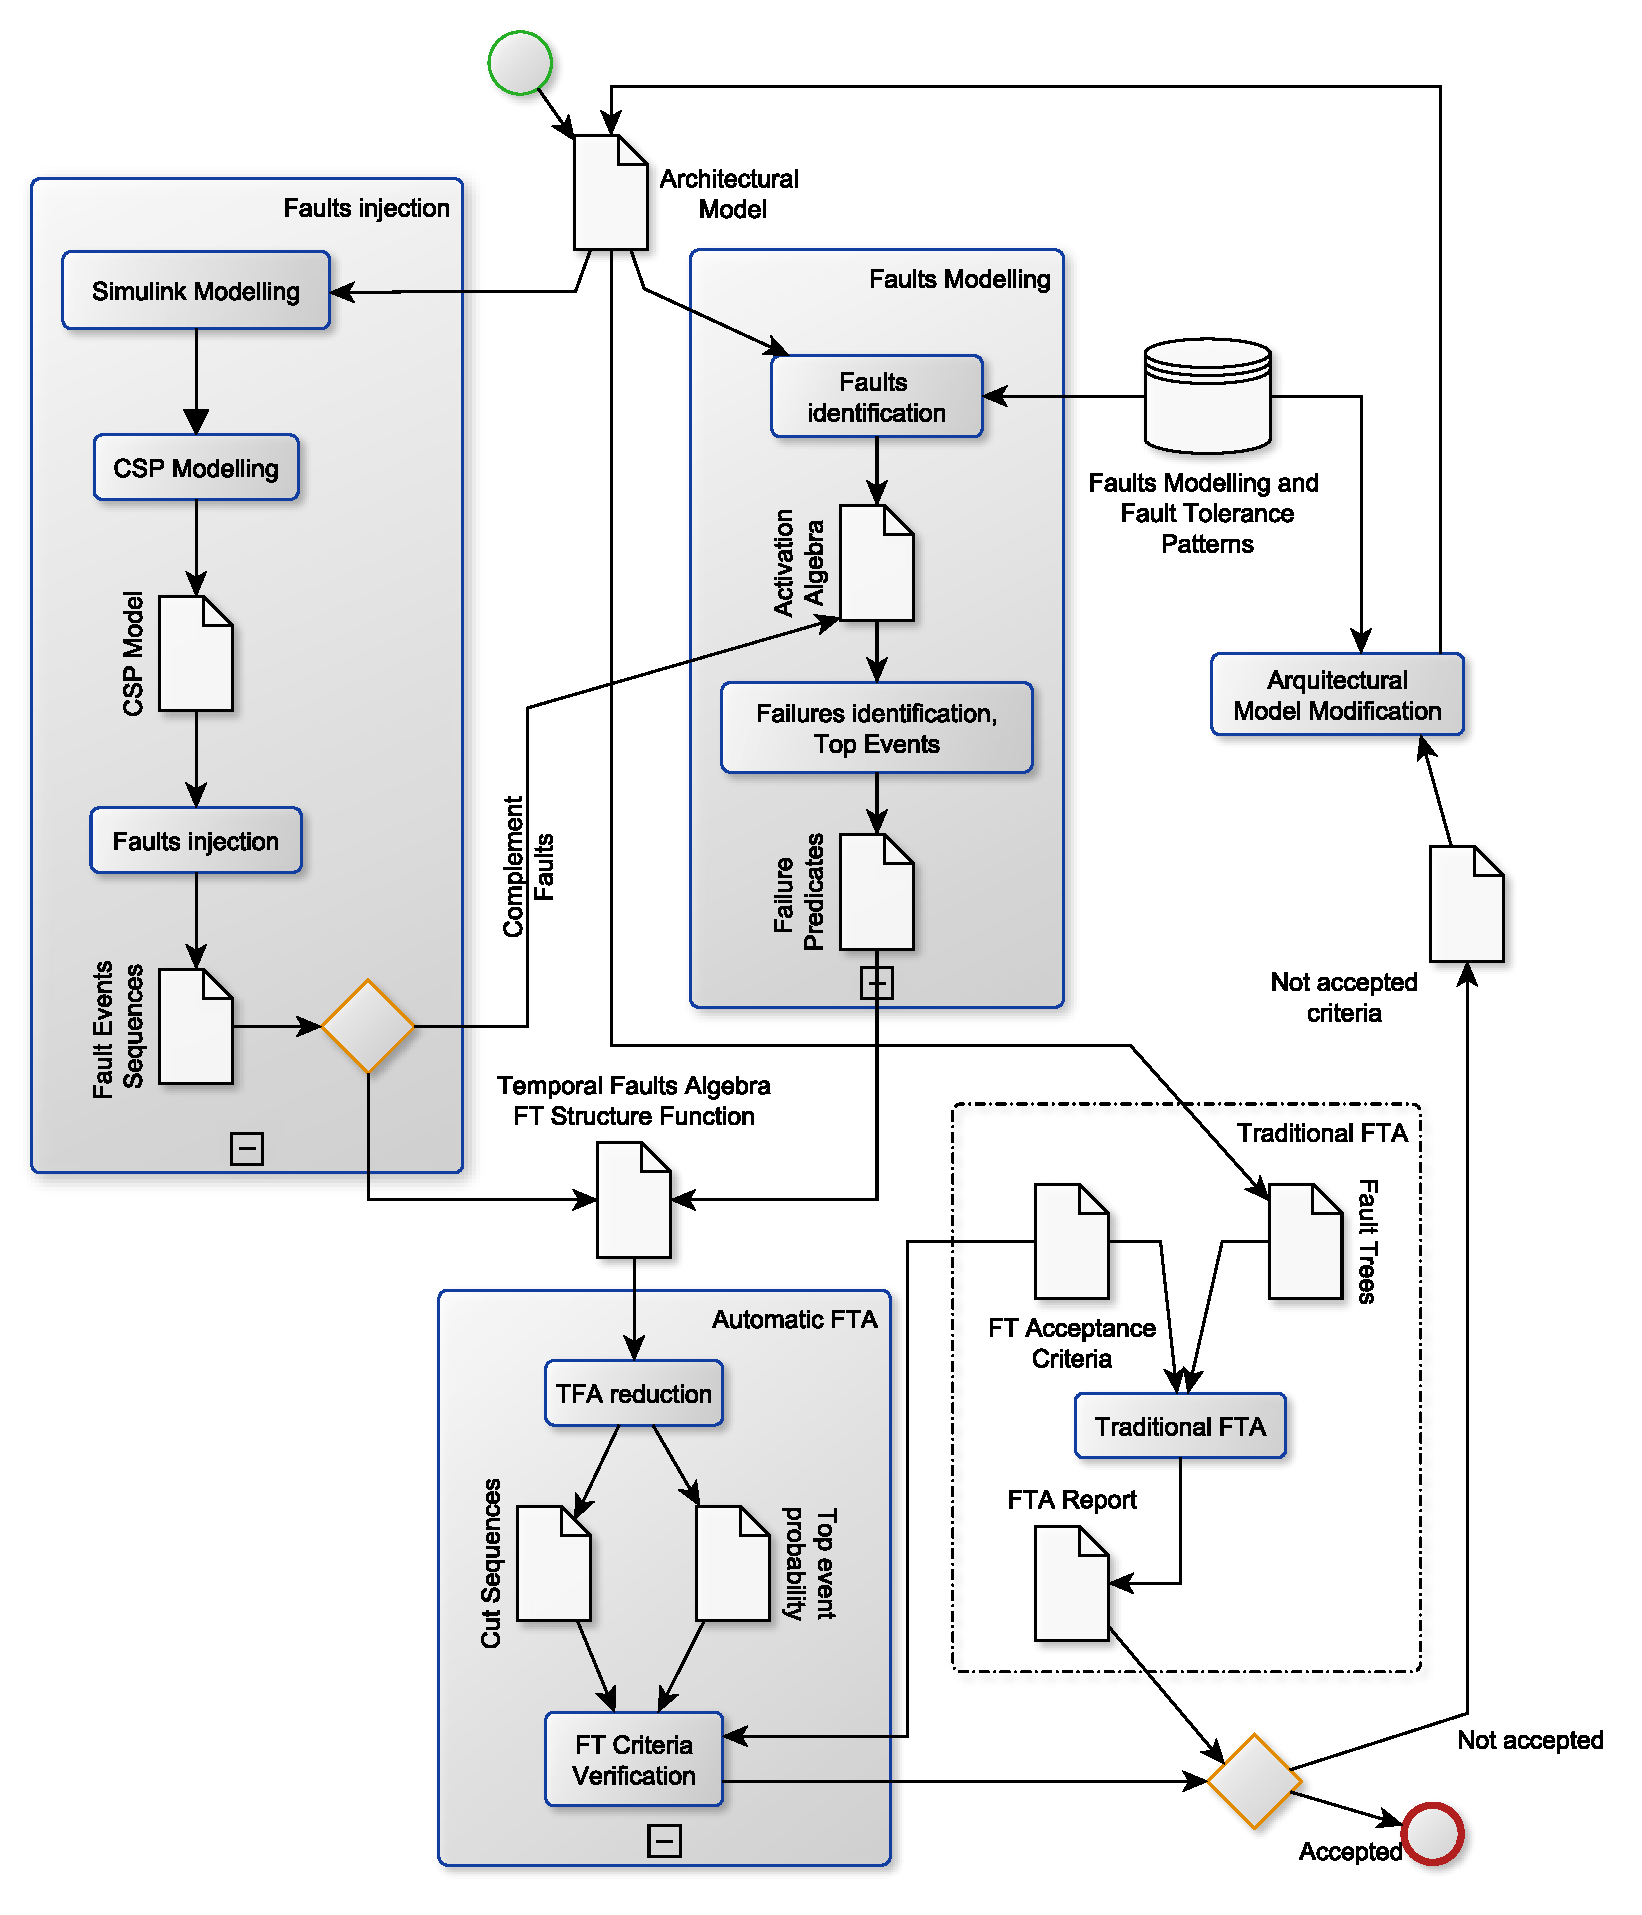
\includegraphics[width=\textwidth]{StrategyOverview}
        \begin{tikzpicture}[overlay, progress/.style={font=\huge}]
        \node<1->[progress] at (3.9,24) {90\%};
        \node<2->[progress] at (15.5,19.2) {0\%};
        \node<3->[progress] at (12.1,22.5) {75\%};
        \node<4->[progress] at (4,10.5) {50\%};
        \node<5->[progress] at (6.7,10.5) {50\%};
        \node<6->[progress] at (3.5,1.8) {20\%};
        \node<7->[progress] at (0,8.3) {0\%};
        \end{tikzpicture}
    \end{column}
\end{columns}


\end{frame}

